\section{Temporal Discretization and Deviation Evaluation} \label{sec:implementation}
While the previous \cref{sec:theoretical-foundations} dealt with the theoretical foundations surrounding electron holography, interference gating and time-discrete signals, this section, as the main focus of this thesis, details the self-developed method and its various steps to discretize the input signal and evaluate its deviation. This approach provides a quantification of the discretization deviation generally introduced by time resolved measurements like the interference gating method.

The self-developed method can be broken down into two main sections (\cref{fig:flowchart}): While the first part deals with the actual temporal discretization of the input signal (\cref{ssec:discretization-method}), the second part evaluates the deviation between the time-discrete and input signal (\cref{ssec:evaluation-method}).

The temporal discretization step (\cref{fig:flowchart}) is designed in accordance to the interference gating method such that the arbitrary input signal (corresponding to the control signal) is averaged over defined time intervals (corresponding to the gate length $\tau$) at different equidistant time points (corresponding to the sampling resolution $t_0$). The resulting deviations depend (as described in \cref{ssec:discrete-signals}) on the temporal discretization parameters $\tau$ and $t_0$ and are quantified in the evaluation part (\cref{fig:flowchart}). The self-developed method allows for predictions to be made about an appropriate choice of measurement parameters $\tau$ and $t_0$ for time-resolved measurements using interference gating for different control signals.%
\begin{figure}[H]
	\centering
	\begin{tikzpicture}
	\tikzstyle{startstop} = [rectangle,rounded corners,minimum width=3cm,minimum height=1cm,text centered,draw=none,fill=blue!30,align=center]
	\tikzstyle{error} = [ellipse,minimum width=3cm,minimum height=1cm,text centered,draw=none,fill=red!30,align=center]
	\tikzstyle{process} = [rectangle,minimum width=3cm,minimum height=1cm,text centered,draw=none,fill=orange!30,align=center]
	\tikzstyle{decision} = [trapezium,trapezium left angle=70,trapezium right angle=110,minimum width=3cm,minimum height=1cm,text centered,draw=none,fill=green!30,align=center]

	\matrix[matrix of nodes, nodes in empty cells, column sep=0.6cm, row sep=1cm, anchor=center, nodes={anchor=center}]{
	\node (start) [startstop] {Input Data}; &
	\node (split) [process] {Split Data}; &
	\node (length) [decision] {Intervals \\ Equally Sized?}; &
	\node (average) [process] {Average \\ Intervals};\\
	& & \node (warning) [error] {Output \\ Warning}; & \\
	\node (average-dev) [startstop] {Normalize Average \\ Deviation}; &
	\node (calc-dev) [process] {Calculate Single \\ Deviations}; &
	\node (spline-data) [process] {Input Data \\ into Spline}; &
	\node (spline) [process] {Construct \\ Cubic Spline};\\};
	\draw [thick,->,>=stealth] (start) -- (split);
	\draw [thick,->,>=stealth] (split) -- (length);
	\draw [thick,->,>=stealth] (length) -- node[left] {\textsc{no}} (warning);
	\draw [thick,->,>=stealth] (length) -- node[below] {\textsc{yes}} (average);
	\draw [thick,->,>=stealth] (warning) -- (average);
	\draw [thick,->,>=stealth] (average) -- (spline);
	\draw [thick,->,>=stealth] (spline) -- (spline-data);
	\draw [thick,->,>=stealth] (spline-data) -- (calc-dev);
	\draw [thick,->,>=stealth] (calc-dev) -- (average-dev);
	\draw [ultra thick, draw=cyan, fill=white, fill opacity=0, rounded corners] (-7.8,-1.2) rectangle (7.8,3.2);
	\draw [ultra thick, draw=magenta, fill=white, fill opacity=0, rounded corners] (-7.8,-3.2) rectangle (7.8,-1.4);
	\node [text=cyan] (l1) at (0,3.5) {\textbf{Temporal Discretization}};
	\node [text=magenta] (l2) at (0,-3.5) {\textbf{Deviation Evaluation}};
\end{tikzpicture}%
	\caption{Flowchart outlining the various steps of the temporal discretization and deviation evaluation method. The flowchart can be broken down into two main sections: The first part (outlined in cyan) deals with the actual discretization of the input signal by splitting it into equally sized intervals and averaging over them, whereas the second part (outlined in magenta) evaluates the deviation between the time-discrete signal and the input signal at every data point by means of a cubic spline interpolation.}
	\label{fig:flowchart}
\end{figure}
Even though various different methods for comparing, and especially evaluating the deviation between, different signals have been developed throughout the years, most approaches are only optimized for certain types of signals under certain restrictions and yield subpar results otherwise \cite{Bellman1959,Flores1986,Makridakis1993,Elmore2001,Hyndman2006,Kennedy2007,Kim2016}. To be precise, these methods are either unsuitable for signals of different length or sampling resolution, cannot be applied to signals that feature values that are (near) zero or are confined to non-intuitive or limited scales \cite{Bellman1959,Flores1986,Makridakis1993,Elmore2001,Hyndman2006,Kennedy2007,Kim2016}.

The presented method addresses these kinds of problems by applying a more generalized approach suitable for a wide range of signals without imposing unnecessary constrains. In detail, the use of cubic spline interpolation allows for the comparison of signals with non-matching and arbitrary lengths or sampling resolutions, while normalizing the deviation to the peak-to-peak amplitude avoids undefined cases or numerical instability. 
\subsection{Temporal Discretization Method} \label{ssec:discretization-method}
The temporal discretization step of the self-developed method is intended to emulate the measurement process of time-resolved techniques (e.\,g. interference gating). In contrast to the sample and hold method described in \cref{eq:sample-and-hold-time}, this approach averages over a time interval $\tau$ instead of simply locking at a constant value.

The temporal discretization of the input signal is achieved in multiple steps. Starting with the input signal $U\left(t\right)$ as a set of $k$ discrete data points, both the time values $t_i$ and the voltage values $U_i$, with $i \in \mathbb{N}$ and $i \leq k$, are split in equally\footnote{If the chosen combination of interval size and interval spacing leads to non-integer sized intervals, the last interval is truncated in such a manner that the specified parameters can still be realized and the user is warned.} sized intervals, representing the gate length $\tau$, with equal spacing, representing the sampling resolution $t_0$, in between. Those intervals are then averaged, leading to $n$ time-discrete data points $\overline{U}_j\left(t_{g_j}\right)$ for $n$ intervals (\cref{fig:discretization-method}). If the time values $t_i$ are all uniformly sampled, the averaged time $t_{g_j}$ is just the median of the current interval.

This approach poses one problem: Selecting a gate length $\tau$ that is large relative to the period length $T$ (e.\,g. $\tau = 0.5T$) would position the first time-discrete data point far into the signal, effectively truncating the interpolated time-discrete signal, and therefore the domain for the deviation evaluation, compared to the input signal. This means that comparing both signals would be limited to the length of the shorter interpolated time-discrete signal. In order to circumvent this restriction, the signal is artificially extended to multiple periods, or the input signal that is provided is already of sufficient length, and time discretized and interpolated over those multiple (at least three) periods. The deviation between both signals is then only evaluated at a single period $T$ that is not the first or last one, effectively extending the domain for the deviation evaluation to a full period $T$ of the input signal, including the edges.%
\begin{figure}[H]
	\centering
	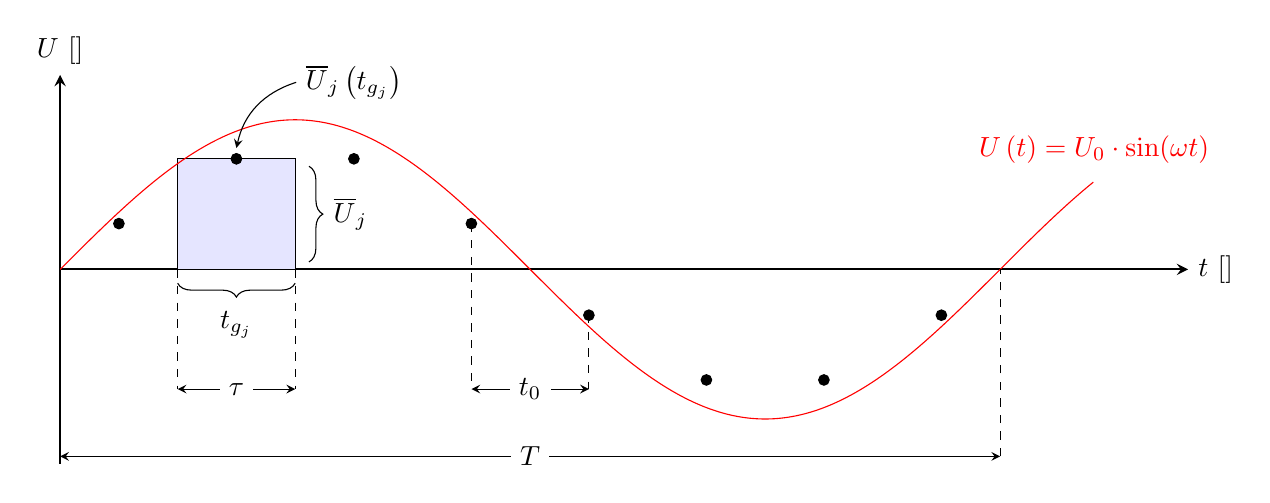
\begin{tikzpicture}[domain=0:2.2*pi, samples=500, scale=1.9, smooth]
	\draw [thick,->,>=stealth] (0,0) -- (2.4*pi,0) node[right] {$t$ $\left[\si{\second}\right]$};
	\draw [thick,->,>=stealth] (0,-1.3) -- (0,1.3) node[above] {$U$ $\left[\si{\volt}\right]$};
	\filldraw [fill=blue!10,draw=black] (2/8*pi, 0) rectangle (4/8*pi, {sin(3/8*pi r)*0.8});
	\draw [red] plot (\x, {sin(\x r)});
	\draw [decorate,decoration={brace,amplitude=5pt,mirror,raise=5pt}]
	(2/8*pi,0) -- (4/8*pi,0) node[midway,yshift=-20pt]{$t_{g_j}$};
	\draw [decorate,decoration={brace,amplitude=5pt,mirror,raise=5pt}]
	(4/8*pi,0.05) -- (4/8*pi,{sin(3/8*pi r)*0.8-0.05}) node[midway,xshift=20pt]{$\overline{U}_j$};
	\node (l1) at (5/8*pi,1.25) {$\overline{U}_j\left(t_{g_j}\right)$};
	\node[text=red] (l2) at (2.2*pi,0.8) {$U\left(t\right) = U_0 \cdot \sin(\omega t)$};
	\node [fill=black,circle,inner sep=0pt,outer sep=0pt, minimum size=4pt] (c1) at (3/8*pi,{sin(3/8*pi r)*0.8}) {};
	\draw[dashed] (2/8*pi, 0) -- (2/8*pi, -0.8);
	\draw[dashed] (4/8*pi, 0) -- (4/8*pi, -0.8);
	\draw[dashed] (2*pi, -1.25) -- (2*pi, 0);
	\draw[dashed] (7/8*pi,{sin(7/8*pi r)*0.8}) -- (7/8*pi,-0.8);
	\draw[dashed] (9/8*pi,{sin(9/8*pi r)*0.8}) -- (9/8*pi,-0.8);
	\draw[<->,>=stealth] (2/8*pi, -0.8) -- (4/8*pi, -0.8) node [midway, fill=white] {$\tau$};
	\draw[<->,>=stealth] (7/8*pi, -0.8) -- (9/8*pi, -0.8) node[midway,fill=white] {$t_0$};
	\draw[<->,>=stealth] (0, -1.25) -- (2*pi, -1.25)  node [midway, fill=white] {$T$};
	\draw[->,>=stealth,bend angle=30,bend right] (l1.west) to node {} ([yshift=1pt] c1.north);
	\filldraw (1/8*pi,{sin(1/8*pi r)*0.8}) circle (1pt);
	\filldraw (3/8*pi,{sin(3/8*pi r)*0.8}) circle (1pt);
	\filldraw (5/8*pi,{sin(5/8*pi r)*0.8}) circle (1pt);
	\filldraw (7/8*pi,{sin(7/8*pi r)*0.8}) circle (1pt);
	\filldraw (9/8*pi,{sin(9/8*pi r)*0.8}) circle (1pt);
	\filldraw (11/8*pi,{sin(11/8*pi r)*0.8}) circle (1pt);
	\filldraw (13/8*pi,{sin(13/8*pi r)*0.8}) circle (1pt);
	\filldraw (15/8*pi,{sin(15/8*pi r)*0.8}) circle (1pt);
\end{tikzpicture}%
	\caption{Graph illustrating the temporal discretization of the input signal $U\left(t\right)$: The input signal is averaged, both in time $t_{g_j}$ and voltage $\overline{U}_j$, resulting in time-discrete data points $\overline{U}_j\left(t_{g_j}\right)$. The width of the interval represent the gate length $\tau$, the distance between them the sampling resolution $t_0$.}
	\label{fig:discretization-method}
\end{figure}
This approach allows for a flexible adjustment of both the gate length $\tau$ and the sampling resolution $t_0$, thus preserving the implementation of the interference gating method detailed in \cref{ssec:igate}, while still being suitable for a wide range of signals. Furthermore, averaging over both the time $t$ and the voltage $U$ takes into account the trend of the signal over the whole interval, unlike the sample and hold method described in \cref{eq:sample-and-hold-time} that only considers the signal at a single point $t_i$ in time.

Depending on the discretization parameters $\tau$ and $t_0$, this results in inherent deviations from the input signal, which affect the accuracy of real measurements (e.\,g. interference gating) when investigating dynamic processes. In the deviation evaluation step (\cref{ssec:evaluation-method}), these deviations are quantified in order to subsequently make a suitable choice of parameters $\tau$ and $t_0$.
\subsection{Deviation Evaluation Method} \label{ssec:evaluation-method}
In order to evaluate the deviation between the time-discrete data points from the previous step and the input signal, the $n$ time-discrete data points are interpolation with a cubic spline $S$ \cite{Dyer2001}, resulting in the interpolated time-discrete signal $U_S\left(t\right)$ (\cref{fig:evaluation-method}). This method allows for a comparison at every time point $t_i$ of the input signal while still guaranteeing that \cite{Dyer2001}:
\begin{itemize}
	\item The reconstructed curve goes through all $n$ time-discrete data points, the so called \emph{knots}, therefore satisfying $S\left(t_{g_j}\right) = \overline{U}_j$.
	\item The $n$ knots are connected by $n-1$ piecewise cubic polynomials, avoiding problems such as \emph{Runge's phenomenon} \cite{Runge1901}.
	\item The resulting spline $S \in C^2$ is twice continuously differentiable by requiring that the first and second derivatives $S'_l\left(t_{g_j}\right) = S'_{l-1}\left(t_{g_j}\right)$ and $S''_l\left(t_{g_j}\right) = S''_{l-1}\left(t_{g_j}\right)$ match for all $n$ knots, resulting in a function that is smooth at all points, including where two polynomials meet.
\end{itemize}
Furthermore, cubic spline interpolation in the time domain $t$ leads to lower deviations than nearest neighbour and linear interpolation \cite{Hussain2015} while avoiding ringing effects encountered in sinc interpolation through zero padding in the frequency domain $f$ \cite{Yaroslavsky1996}. Additionally, the use of cubic spline interpolation allows the self-developed method to be independent of temporal offsets of the input signal.

The reason for interpolating the $n$ time-discrete data points instead of directly comparing them with the input signal can be shown with a simple example:

Setting the gate length $\tau$ to a single data point, thus not actually averaging over an interval but simply picking the corresponding value in the input signal, while setting the sampling resolution to $t_0 = 0.5T$ of the period length $T$ would yield a deviation of zero, even though only two data points can hardly describe non-sinusoidal signal perfectly.%
\begin{figure}[H]
	\centering
	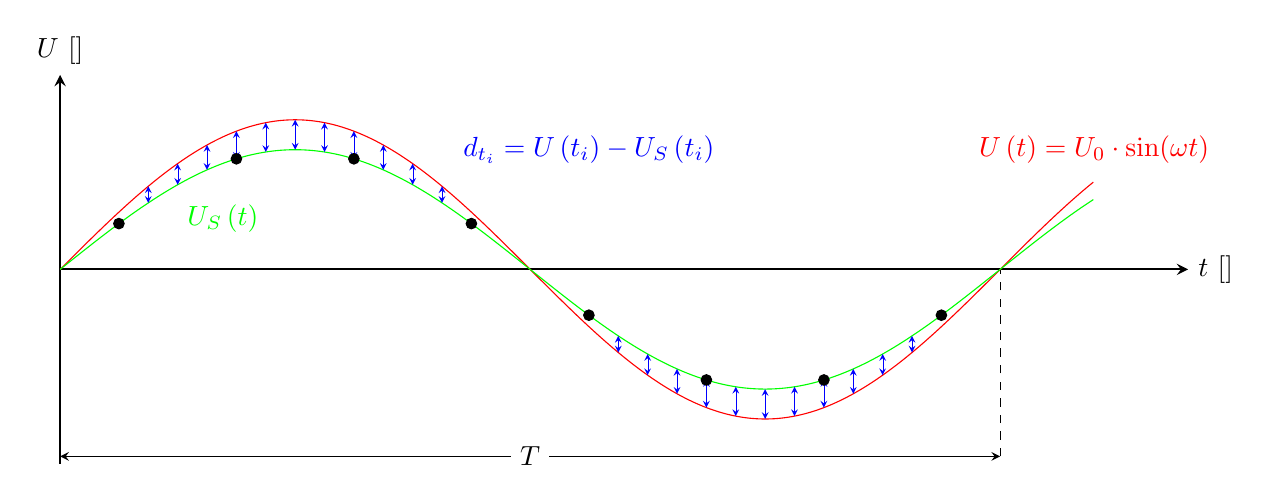
\begin{tikzpicture}[domain=0:2.2*pi, samples=500, scale=1.9, smooth]
	\draw [thick,->,>=stealth] (0,0) -- (2.4*pi,0) node[right] {$t$ $\left[\si{\second} \right]$};
	\draw [thick,->,>=stealth] (0,-1.3) -- (0,1.3) node[above] {$U$ $\left[\si{\volt}\right]$};
	\draw[dashed] (2*pi, -1.25) -- (2*pi, 0);
	\draw[<->,>=stealth] (0, -1.25) -- (2*pi, -1.25)  node [midway, fill=white] {$T$};
	\draw [red] plot (\x, {sin(\x r)});
	\draw [green] plot (\x, {sin(\x r)*0.8});
	\node[text=red] (l1) at (2.2*pi,0.8) {$U\left(t\right) = U_0 \cdot \sin(\omega t)$};
	\node[anchor=north west,text=green] (l2) at (1/4*pi,0.5) {$U_S\left(t\right)$};
	\node[text=blue] (l3) at (9/8*pi,0.8) {$d_{t_i} = \abs{U\left(t_i\right) - U_S\left(t_i\right)}$};
	\foreach \x in {0.1875,0.25,...,0.8125}{
		\draw [ultra thin, <->, >=stealth, blue] ({\x*pi},{sin(\x*pi r)*0.8}) -- ({\x*pi},{sin(\x*pi r)});}
	\foreach \x in {1.1875,1.25,...,1.8125}{
		\draw [ultra thin, <->, >=stealth, blue] ({\x*pi},{sin(\x*pi r)*0.8}) -- ({\x*pi},{sin(\x*pi r)});}
				\filldraw (1/8*pi,{sin(1/8*pi r)*0.8}) circle (1pt);
	\filldraw (3/8*pi,{sin(3/8*pi r)*0.8}) circle (1pt);
	\filldraw (5/8*pi,{sin(5/8*pi r)*0.8}) circle (1pt);
	\filldraw (7/8*pi,{sin(7/8*pi r)*0.8}) circle (1pt);
	\filldraw (9/8*pi,{sin(9/8*pi r)*0.8}) circle (1pt);
	\filldraw (11/8*pi,{sin(11/8*pi r)*0.8}) circle (1pt);
	\filldraw (13/8*pi,{sin(13/8*pi r)*0.8}) circle (1pt);
	\filldraw (15/8*pi,{sin(15/8*pi r)*0.8}) circle (1pt);
\end{tikzpicture}%
	\caption{Graph illustrating the deviation evaluation between the interpolated time-discrete signal $U_S\left(t\right)$ and input signal $U\left(t\right)$: The time-discrete data points $\overline{U}_j\left(t_{g_j}\right)$ are interpolated with a cubic spline $S$, so the resulting absolute difference $d_{t_i}$ between both signals can be calculated at every time point $t_i$.}
	\label{fig:evaluation-method}
\end{figure}
After interpolating the $n$ time-discrete data points with a cubic spline, all input time values $t_i$ can be input into the spline, allowing to calculate the absolute deviation $d_{t_i} = \abs{U\left(t_i\right) - U_S\left(t_i\right)}$ between the interpolated time-discrete signal $U_S\left(t\right)$ and the input signal $U\left(t\right)$ at every time point $t_i$. In order to give an intuitive, single measurement of the deviation, all absolute deviations $d_{t_i}$ are summed up and averaged, yielding: $$\overline{d} = \frac{1}{k}\sum^k_{i=1}d_{t_i}.$$ 
To ensure easy comparability between different signals, the averaged absolute deviation $\overline{d}$ can be normalized to the peak-to-peak amplitude $U_{pp} = \abs{U_{max}-U_{min}}$, resulting in: $$\overline{d}_{pp} = \frac{\overline{d}}{U_{pp}}.$$ 
This approach, unlike those mentioned at the beginning of \cref{sec:implementation}, does not suffer from flaws such as being undefined for values that are zero, placing heavier penalties on negative deviations than on positive deviations, having a maximum deviation of 100\%, yielding extremely high deviations for small values or being confined to a non-intuitive or limited scale \cite{Bellman1959,Flores1986,Makridakis1993,Elmore2001,Hyndman2006,Kennedy2007,Kim2016}.
\subsection{Discretization and Evaluation of Real Signals} \label{ssec:real-signals}
A particular advantage of the self-developed method is its universal application to various types of input signal. Moreover, like the investigation of physical processes, which can feature various types of dynamics (e.\,g. linear, quadratic, exponential), the generalized approach of the self-developed method allows for the investigation of different input signals.

The following subsection discusses the results from the above described method for three different signals: a sine wave, a square wave and a Bat-Signal. All $m$ deviations $\overline{d}_{pp}$, with $m$ denoting the number of possible combinations of gate length $\tau$ and sampling resolution $t_0$, which are provided relative to the period length $T$ of the respective signal, are normalized to the peak-to-peak amplitude $U_{pp}$ as specified in \cref{ssec:evaluation-method}.
\subsubsection{Sine Wave Signal} \label{sssec:sine-wave}
Starting with a sine wave signal, an exemplary plot showcasing the temporal discretization method can be seen in \cref{fig:sine-real-i2000-s1000}. Here, the gate length of $\tau = 0.2T$ is represented by the light blue bars, which overlap due to the choice of sampling resolution $t_0 = 0.1T$. 
\begin{figure}[H]
	\centering
	\includegraphics[width=0.75\textwidth]{Figures/Signals/sine_real_i2000_s1000.pdf}
	\caption{Plot of the oscilloscope sine wave signal $U\left(t\right)$ along with the (overlapping) intervals over whom are averaged, the time-discrete data points $\overline{U}_j\left(t_{g_j}\right)$ and the interpolated time-discrete signal $U_S\left(t\right)$ for a gate length of $\tau = 0.2T$ and a sampling resolution of $t_0 = 0.1T$.}
	\label{fig:sine-real-i2000-s1000}
\end{figure}
Both the gate length $\tau$ and the sampling resolution $t_0$ can subsequently be set to values in an interval of $\tau, t_0 \in \interval[scaled, open left]{0}{0.5T}$, where $m$, the number of possible combinations, depends on the chosen step size of $\tau$ and $t_0$. The $m$ different deviations $\overline{d}_{pp}$ can then be calculated and plotted in two dimensions (\cref{fig:sine-real-combination}), revealing two interesting conclusions:
\begin{itemize}
	\item In order to achieve a deviation of $\overline{d}_{pp} < 5\%$, both the gate length $\tau$ and the sampling resolution $t_0$ can be set to values up to $\tau = t_0 \approx 0.3T$.
	\item A gate length of $\tau = 0.1T$ and a sampling resolution of $t_0 = 0.05T$, which is easily within experimental feasibility, yield a deviation of $\overline{d}_{pp} < 1\%$.
\end{itemize}
This shows that signals which do not feature rapid changes in amplitude or slope over small intervals can be sampled with gate lengths $\tau$ and sampling resolutions $t_0$ beyond $0.1T$ while still resulting in a time-discrete signal that is representative of the oscilloscope signal (i.\,e. low single digit deviation $\overline{d}_{pp}$).
\begin{figure}[H]
	\centering
	\includegraphics[width=0.5\textwidth]{Figures/Combinations/sine_real.pdf}
	\caption{Two-dimensional plots showcasing the $m$ different deviations $\overline{d}_{pp}$ of the sine wave signal for different combinations of gate length $\tau$ and sampling resolution $t_0$, where both parameters are set to $\tau, t_0 \in \interval[scaled, open left]{0}{0.5T}$, with dashed contour lines for $\overline{d}_{pp} = 0.01, \dotsc ,0.05$.}
	\label{fig:sine-real-combination}
\end{figure}
It should be noted that setting the gate length close to one sampling point while choosing a sampling resolution of $t_0 = 0.5T$ leads to a deviation of $\overline{d}_{pp} > 30\%$, which is reflected in the yellow artifact region in \cref{fig:sine-real-combination}. This is caused by the fact that such a small gate length $\tau$ is effectively equivalent to the corresponding value in the oscilloscope signal, which is (near) zero for a sine wave signal and a sampling of resolution of $t_0 = 0.5T$. The resulting time-discrete data points are therefore all (near) zero as well, yielding an interpolated time-discrete signal that is effectively a straight line of slope zero. Lowering the sampling resolution to just $t_0 = 0.4T$ mitigates most of this since the intervals are now positioned at non-zero values for the sine wave signal.
\subsubsection{Square Wave Signal} \label{sssec:square-wave}
Switching from a sine wave to a square wave signal (\cref{fig:square-real-i50-s25}), the same two dimensional plot showcasing the deviation $\overline{d}_{pp}$ of $m$ different combinations of gate length $\tau$ and sampling resolution $t_0$ can be calculated (\cref{fig:square-real-combination}). This shows that the same deviation of $\overline{d}_{pp} < 5\%$ requires a gate length of $\tau < 0.15T$ and a sampling resolution of $t_0 < 0.1T$. Furthermore, a gate length of $\tau = 0.1T$ and sampling resolution of $t_0 = 0.05T$, which is easily within experimental feasibility, results in a deviation of $\overline{d}_{pp} \approx 3\% - 4\%$, three to four times that of the sine wave signal.

Examining \cref{fig:square-real-i50-s25}, for which a gate length of $\tau = 0.1T$ and sampling resolution of $t_0 = 0.05T$ was used, reveals that, even-though the deviation $\overline{d}_{pp}$ is two to three times higher than the sine wave signal, the interpolated time-discrete signal is still an accurate representation of the oscilloscope square wave signal.
\begin{figure}[H]
	\centering
	\includegraphics[width=0.75\textwidth]{Figures/Signals/square_real_i50_s25.pdf}
	\caption{Plot of the oscilloscope square wave signal $U\left(t\right)$ along with the (overlapping) intervals over whom are averaged, the time-discrete data points $\overline{U}_j\left(t_{g_j}\right)$ and the interpolated time-discrete signal $U_S\left(t\right)$ for a gate length of $\tau = 0.1T$ and a sampling resolution of $t_0 = 0.05T$.}
	\label{fig:square-real-i50-s25}
\end{figure}
A large contribution to the deviation $\overline{d}_{pp}$ stems from not only the noise of the oscilloscope signal causing small deviations at every data point, but also from the sections of sharp rise and fall in both signals. Nevertheless, pushing the gate length $\tau$ and sampling resolution $t_0$ both beyond $0.15T$ quickly results in two digit deviations $\overline{d}_{pp}$, a sharp contrast to the observations of the sine wave signal from \cref{sssec:sine-wave}.
\begin{figure}[H]
	\centering
		\centering
	\includegraphics[width=0.75\textwidth]{Figures/Combinations/square_real.pdf}
	\caption{Two-dimensional plots showcasing the $m$ different deviations $\overline{d}_{pp}$ of the square wave signal for different combinations of gate length $\tau$ and sampling resolution $t_0$, where both parameters are set to $\tau, t_0 \in \interval[scaled, open left]{0}{0.5T}$, with dashed contour lines for $\overline{d}_{pp} = 0.01, \dotsc ,0.05$.}
	\label{fig:square-real-combination}
\end{figure}
\subsubsection{Bat-Signal} \label{sssec:Bat-Signal}
In order to test the validity of the self-developed method regarding complicated signals with rapid and frequent changes in amplitude, as they often occur in physical processes and measurements, the same temporal discretization and deviation evaluation can be applied to a more complicated Bat-Signal (\cref{fig:batman-real-i500-s250}). The deviation $\overline{d}_{pp}$ for $m$ different combinations of gate length $\tau$ and sampling resolution $t_0$ can be calculated and plotted in two dimensions in much the same way, resulting in \cref{fig:batman-real-combination}. It is apparent that the same deviation of $\overline{d}_{pp} < 5\%$ requires even lower values for the parameters (i.\,e. a gate length of $\tau < 0.1T$ and a sampling resolution of $t_0 < 0.05T$). This also means that those parameters, which are easily within experimental feasibility, yield a deviation of $\overline{d}_{pp} \approx 5\%$, which is not only around four times higher than the sine wave signal, but also around one-fourth to one-third higher than the deviation of the square wave signal.
\begin{figure}[H]
	\centering
	\includegraphics[width=0.75\textwidth]{Figures/Signals/batman_real_i500_s250.pdf}
	\caption{Plot of the oscilloscope Bat-Signal $U\left(t\right)$ along with the (overlapping) intervals over whom are averaged, the time-discrete data points $\overline{U}_j\left(t_{g_j}\right)$ and the interpolated time-discrete signal $U_S\left(t\right)$ for a gate length of $\tau = 0.05T$ and a sampling resolution of $t_0 = 0.025T$.}
	\label{fig:batman-real-i500-s250}
\end{figure}
The Bat-Signal is a perfect example of a complicated signal with rapid changes in amplitude and slope. The signal not only features sections with little change in trend, but also those of sharp and sudden rise or decline (such as the spikes around the middle). It is these areas where the attenuating effect of the averaging approach to the amplitude is particularly apparent, especially with increasing gate length $\tau$.
\begin{figure}[H]
	\centering
		\centering
	\includegraphics[width=0.75\textwidth]{Figures/Combinations/batman_real.pdf}
	\caption{Two-dimensional plots showcasing the $m$ different deviations $\overline{d}_{pp}$ of the Bat-Signal for different combinations of gate length $\tau$ and sampling resolution $t_0$, where both parameters are set to $\tau, t_0 \in \interval[scaled, open left]{0}{0.5T}$, with dashed contour lines for $\overline{d}_{pp} = 0.01, \dotsc ,0.05$.}
	\label{fig:batman-real-combination}
\end{figure}
\subsection{Discussion} \label{ssec:implementation-discussion}
The previous sections presented a method to investigate the inherent discretization deviations of time-resolved measurement processes. This especially allows the prediction of suitable measurement parameters $\tau$ and $t_0$ within specified error limits for different dynamic processes (represented by the input signal $U\left(t\right)$). With the temporal discretization step, the measurement process of time-resolved methods (e.\,g. interference gating) could be reproduced exactly, which is a direct implementation of the experiment.

Interpolating the $n$ time-discrete data points with a cubic spline $S \in C^2$ further allows for a comparison of signals with different length or sampling resolution, whereas normalizing the deviation $\overline{d}$ to the peak-to-peak amplitude $U_{pp}$ ensures applicability for values that are (near) zero without numerical instability. Another advantage of the normalized deviation $\overline{d}_{pp}$ is the ability to compare different physical processes with non-matching amplitude $U_{pp}$.

The self-developed method was applied to three different signals, namely a sine wave, square wave and Bat-Signal, in \cref{ssec:real-signals}. Comparing all three signals shows that the gate length $\tau$ and sampling resolution $t_0$ required to achieve a representative output from the interference gating method (i.\,e. a deviation $\overline{d}_{pp}$ of up to $5\%$) is highly dependent on the oscilloscope signal and varies anywhere from up to $\tau = t_0 \approx 0.3T$ for the sine wave signal to as low as $\tau < 0.1T$ and $t_0 < 0.05T$ for the Bat-Signal.

As described in \cref{ssec:discrete-signals}, signals can also be analyzed in the frequency domain $f$ instead of the time domain $t$, as is common in signal theory. As an example, this approach is made for the Bat-Signal to separate it into its frequency components, along with the interpolated time-discrete signal for gate length $\tau$ and sampling resolution $t_0$ set to $\tau = t_0 = 0.1T, \dotsc ,0.5T$, and display the result as a bar plot (\cref{fig:batman-dft}).

Due to its complicated composition, the Bat-Signal features a wide array of frequency components with different spectral amplitudes. To be precise, the frequencies ranging from $\SIrange{1}{5}{\kilo\hertz}$ make up the dominant part of the spectrum, while the frequencies ranging from $\SIrange{6}{14}{\kilo\hertz}$ see a steep fall in spectral amplitude. Any frequency components beyond that are only present to a minor degree.

Two particularly interesting observations can be drawn from this discrete Fourier transform:
\begin{itemize}
	\item The lowpass-filtering-effect is especially apparent for the interpolated time-discrete signals. Whereas a gate length $\tau$ and sampling resolution $t_0$ of $\tau = t_0 = 0.1T$ still yield frequency components of up to $\SI{7}{\kilo\hertz}$, other parameters of $\tau = t_0 = 0.2T, \dotsc ,0.5T$ have a cutoff frequency of $\SI{3}{\kilo\hertz}$.
	\item The change in spectral amplitude $Q$ for different gate lengths $\tau$ and sampling resolutions $t_0$ does not follow any concrete correlation or pattern.
\end{itemize}
\begin{figure}[H]
	\centering
	\includegraphics[width=0.75\textwidth]{Figures/Signals/batman_dft.pdf}
	\caption{Bar plot representing the frequency spectrum of the Bat-Signal using the discrete Fourier transform for the oscilloscope signal $U\left(t\right)$ as well as different interpolated time-discrete signals $U_S\left(t\right)$ with the gate length $\tau$ and sampling resolution $t_0$ set to $\tau = t_0 = 0.1T, \dotsc ,0.5T$.}
	\label{fig:batman-dft}
\end{figure}
It can be drawn from this that a quantitative comparison of different signals in the frequency domain is hardly possible for complicated signals that are made up of a wide array of frequency components. This shows that the self-developed deviation evaluation method in the time domain introduced in \cref{ssec:evaluation-method} is able to quantify the deviation of such discretization approaches, as used by the interference gating method, for arbitrary combinations of gate length $\tau$ and sampling resolution $t_0$, while still being suitable for a wide range of signals, and should thus be the preferred method.

While the results obtained seem promising at first, especially with respect to the prediction of suitable measurement parameters $\tau$ and $t_0$, their validity needs to be verified. For this purpose, comparisons with phase slopes of time-resolved, reconstructed electron waves are established in \cref{sec:application}. 